\kmuttchapter{THEORETICAL BACKGROUND}

%The electronic properties of conventional material such as silicon

\section{Klein tunneling effect}
    Klein tunneling refers to a relativistic particles penetrate through the potential barrier without backscattering.
    These properties was once unique to the high-energy particles, where it can only be observed in the system with high-driven voltage.
    In 2006, this effect is predicted to occur in low-energy system of graphene \cite{Katsnelson2006a}.
    This is because the electron in graphene mimics the relativistic massless Dirac particle and obey massless Dirac equation,
    which is given by
    \begin{align} \label{2eq:Hamiltonian}
        \hat{H} = -i\hbar v_F \sigma \nabla 
    \end{align}
    where $v_F \approx 10^2 \mathrm{ms^{-1}}$ is Fermi velocity, $\sigma = (\sigma_x, \sigma_y)$ is Pauli matrix. 
    The electron propagation can be modeled as in Fig. \ref{2fig:electron propagation}, consisting of three transport region where the Fermi energy of electron is below the potential barrier.
    By solving Eq. \ref{2eq:Hamiltonian}, the wave function of each region can be expressed as follows
    \begin{equation} \label{2eq:wave function}
        \begin{aligned}
            \psi_1 &= \begin{cases} (e^{ik_x x}+re^{-ik_x x})e^{ik_y y}, &x<0,\\
                (ae^{i q_x x}+be^{-i q_x x})e^{ik_y y},  &0<x<D,\\
                te^{ik_x x + ik_y y},  &x>D,
                \end{cases}\\
            \psi_2 &= \begin{cases} s(e^{ik_x x+i \phi}-re^{-ik_x x-i \phi})e^{ik_y y},  &x<0,\\
                s^\prime(ae^{i q_x x+ i \theta}-be^{-i q_x x- i \theta})e^{ik_y y}, &0<x<D,\\
                ste^{ik_x x + ik_y y+ i \phi}, &x>D,
                \end{cases}
        \end{aligned}
    \end{equation}
    where $k_x = k \cos{\phi}$ and $k_y = k \sin{\phi}$ are x- and y-component wavevector outside the barrier region, respectively.
    $q_x = \sqrt{(E-V_0)^2/(\hbar v_F)^2-k_y^2}$ is x-component wavevector inside the barrier region. 
    $s = \mathrm{sgn}(E)$ and $s^{\prime} = \mathrm{sgn}(E-V_0)$. 
    Since the wave function of each region has to be continuous at the boundary, we can substitute $x = 0$ and $x = D$ to Eq. \ref{2eq:wave function}, which give
    \begin{equation} \label{2eq:boundary condition}
        \begin{aligned}
            1+r-a-b&=0\\
            s(e^{i\phi}-e^{-i\phi}r)-s\prime (e^{i\theta}a-e^{-i\theta}b)&=0\\
            e^{iDq_x}a+e^{-iDq_x}b-e^{iDk_x}t&=0\\
            s \prime (e^{iDq_x+i\theta}a-e^{-iDq_x-i\theta} b)-se^{iDk_x+i\phi}t&=0\\
        \end{aligned}
    \end{equation}
    where r and t is the reflection and transmission coefficient, respectively. Which can be obtained by solving the system of equations above.
    The reflection coefficient has the following expression
    \begin{align} \label{2eq:reflection coefficient}
        r=2ie^{i\phi}\sin{(q_xD)}\times\frac{\sin{\phi}-ss^{\prime}\sin{\theta}}{ss^{\prime}[e^{-iq_xD}\cos{(\phi+\theta)}+e^{iq_xD}\cos{(\phi-\theta)}]-2i\sin{(q_xD)}}
    \end{align}
    Since $T = |t|^2 = 1-|r|^2$, the transmission probability can be expressed as follow
    \begin{align} \label{2eq:transmission probability}
        T = \frac{\cos^2{\phi}}{1-\cos^2{q_x D}\sin^2{\phi}}
    \end{align}
    \begin{figure}[H]
        \centering
        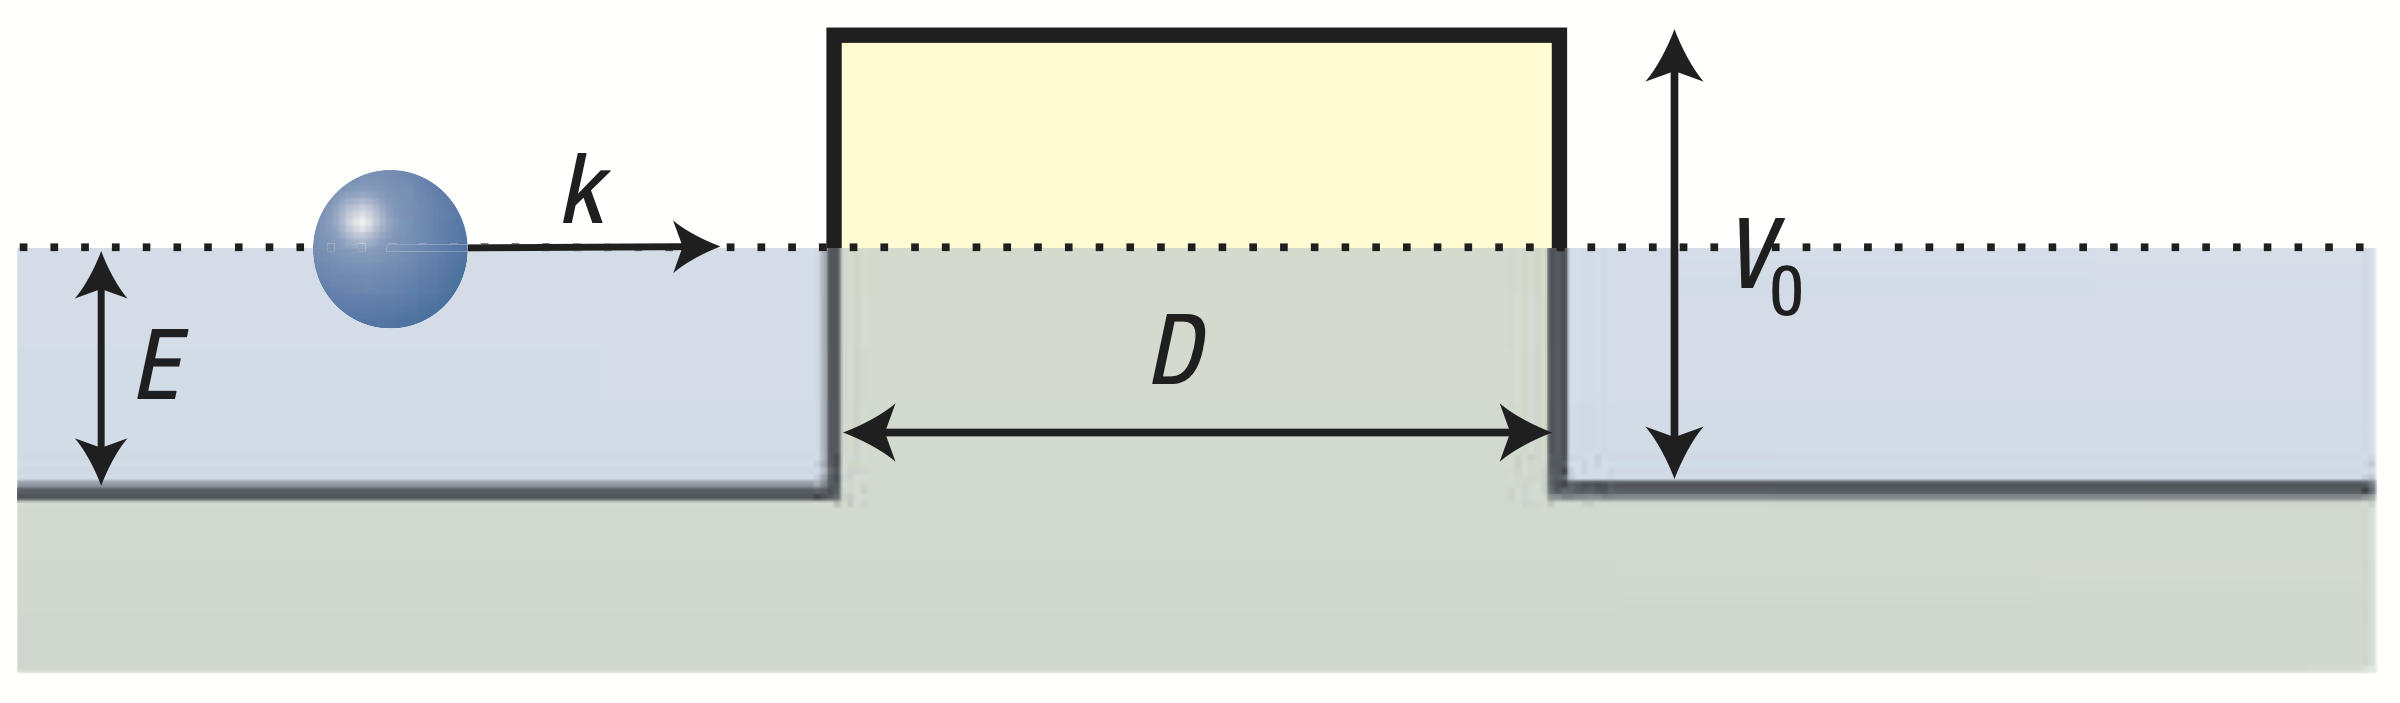
\includegraphics[width=0.7\linewidth]{fig/Chap 2/electron propagation.png}
        \caption{Schematic diagram of electron propagation through the potential barrier of height $V_0$ and width $D$}
        \label{2fig:electron propagation}
    \end{figure}